
\chapter{Anmerkungen zum Format} \label{kap:anmerkungen}


Tabelle \ref{tbl:tab1} zeigt, dass Tabellen eine kursive �berschrift tagen.


\begin{table}[h]
	\centering
	\caption{\textit{So sieht eine Tabelle aus (Bild)}}
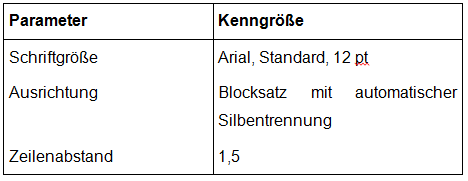
\includegraphics[width=11cm]{img/tabelle.png}
\label{tbl:tab1}
\end{table} 

Tabellen k�nnen entweder als Bild (z.b. aus Excel) eingef�gt werden oder manuell mit LaTeX erstellt werden (siehe \ref{tbl:tab2}):


\begin{table}[h]
	\centering
	\caption{\textit{So sieht eine Tabelle aus (LaTeX)}}	
	\begin{tabular}{|p{3cm}|p{5cm}|}
 			\hline
			\textbf{Parameter} & \textbf{Kenngr��e}\\
			\hline	
				Schriftgr��e & Arial, Standard, 12 pt\\
				Ausrichtung & Blocksatz mit automatischer Silbentrennung\\
				Zeilenabstand & 1,5\\
			\hline
			\end{tabular}
	\label{tbl:tab2}
\end{table} 


Abbildungen tragen eine kursive Bildunterschrift, wie in Abb. \ref{fig:bild1} zu erkennen.

\begin{figure}[ht]
	\centering

\includegraphics[width=8cm]{img/abbildung.png}
\caption{\textit{So sieht eine Abbildung aus}}
\label{fig:bild1}
\end{figure} 

Verweise auf Kapitel, Tabellen oder Abbildungen mit $\backslash ref\{label\}$.

